\chapter{Implementation}
    The proposed project is focused on the design and development of the \emph{Automatic prediction model builder system} in the form of an application with an user-friendly interface, implemented in the cloud environment, and that uses all the principles described in~\ref{analysis}. As the development environment Matlab ecosystem was used.

    \section{Mathematical models}
    The implemented prediction models are based mainly on the principle of linear prediction (LP) and its modifications, such as non-integer linear prediction (fractional-order linear prediction - FLP), LP extended by parameters capable of capturing short-term and long-term trendiness in data (extended linear prediction - ELP), etc., that were developed by the author and his supervisor. These approaches are extended by further statistical methods such as Monte Carlo, Markov chains, etc.
    
        For the identification of the appropriate structure of economic and behavioural models and the identification of the parameters of the selected models, machine learning algorithms are used, which provide the optimal solution for the selected data and thus the use-case.
 
    \section{Application}
    The developed application makes it possible to easily and accurately predict various socioeconomic macro and micro indicators, such as gross/net domestic/national product, economic wealth, unemployment, inflation, average/minimum wage, purchasing power of the population but also the behaviour of customers (customers can also be perceived as households), intended for sectors such as public or state administration, public planning (but also private) finance, banking.
    
    From the point of view of commercial use, a possible application would be predicting the number of customers and the number of orders, the company's income, the success of marketing strategies, or based on the prediction, the planning of the warehouse stocks.

%    \begin{figure}
%        \centering
%        \begin{subfigure}[b]{0.4\textwidth}
%            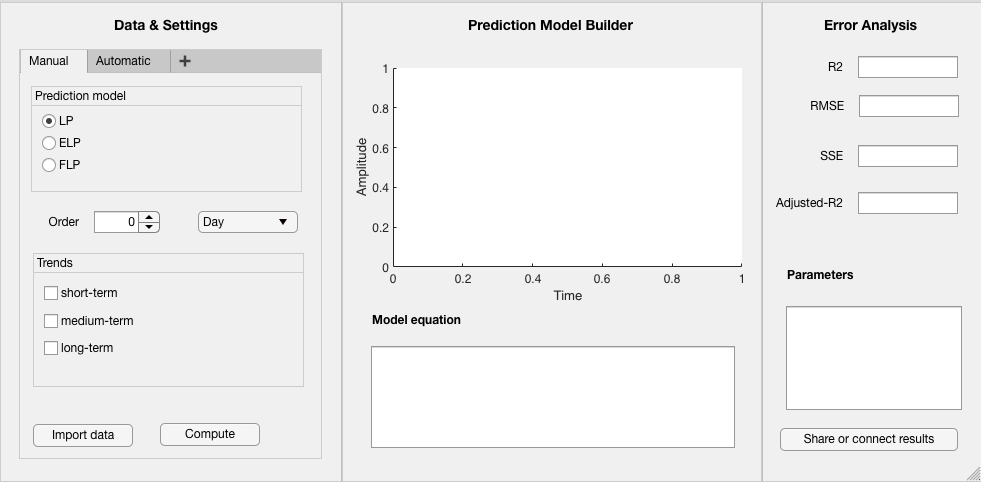
\includegraphics[width=\textwidth]{figures/manual.png}
%            \caption{Manual settings}
%            \label{fig:manual}
%        \end{subfigure}
%        \hspace{0.1\textwidth}
%        \begin{subfigure}[b]{0.4\textwidth}
%            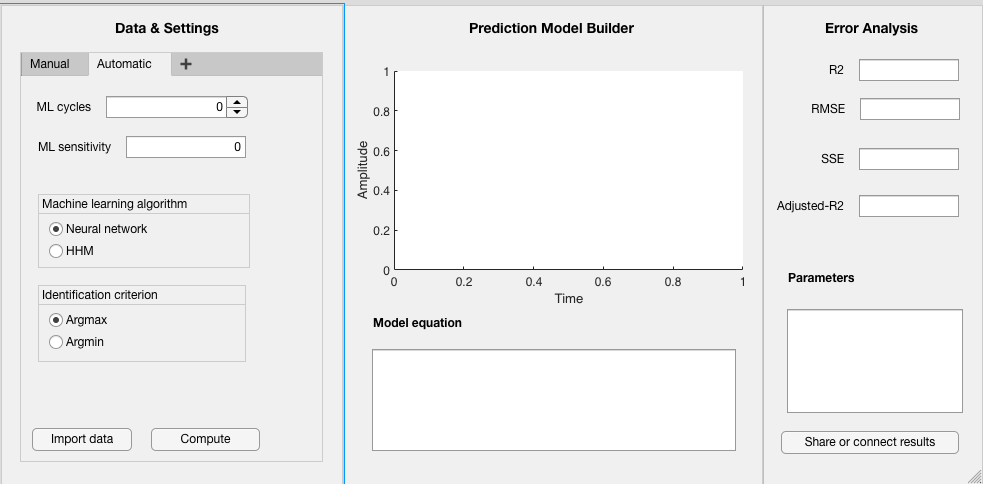
\includegraphics[width=\textwidth]{figures/auto.png}
%            \caption{Automatic settings}
%            \label{fig:automatic}
%        \end{subfigure}
%        \begin{subfigure}[b]{0.4\textwidth}
%            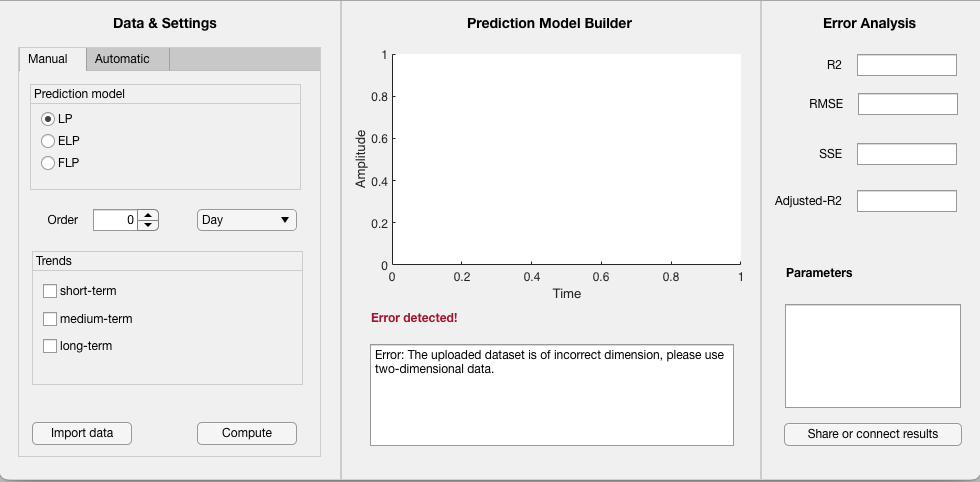
\includegraphics[width=\textwidth]{figures/warning.png}
%            \caption{Dataset warning}
%            \label{fig:warning}
%        \end{subfigure}
%        \hspace{0.1\textwidth}
%        \begin{subfigure}[b]{0.4\textwidth}
%            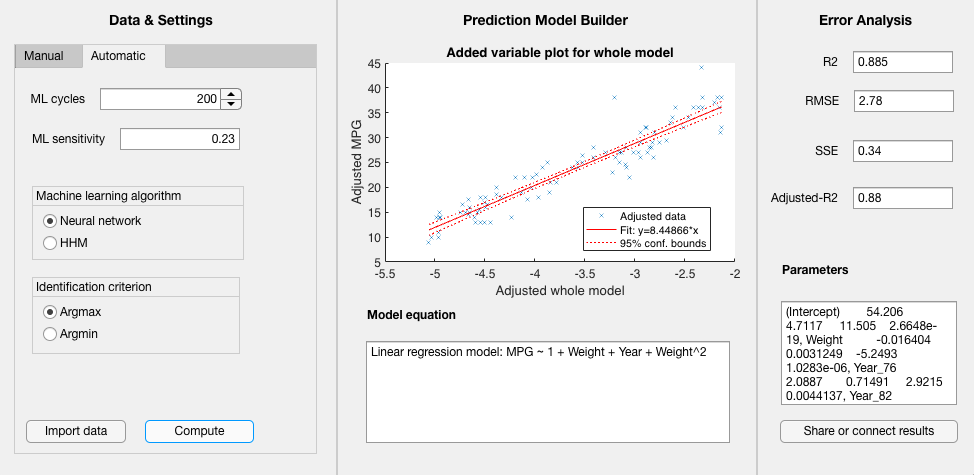
\includegraphics[width=\textwidth]{figures/result.png}
%            \caption{Results}
%            \label{fig:results}
%        \end{subfigure}
%        \label{fig:appoverview}
%        \caption{Application overview}
%    \end{figure}


        \subsection{Dataset import}
 
       To import the dataset to be processed, one has to use the button in the left
        bottom corner~(Fig.~\ref{fig:manual}). Application is able to
        process datasets in *.csv or *.xlsx format. The dataset is firstly checked, if it is of correct format, and in the case of error a warning is shown (Fig.~\ref{fig:warning}) with the tips
        how to format the uploaded dataset.
               \begin{figure}[h!]
        \centering
            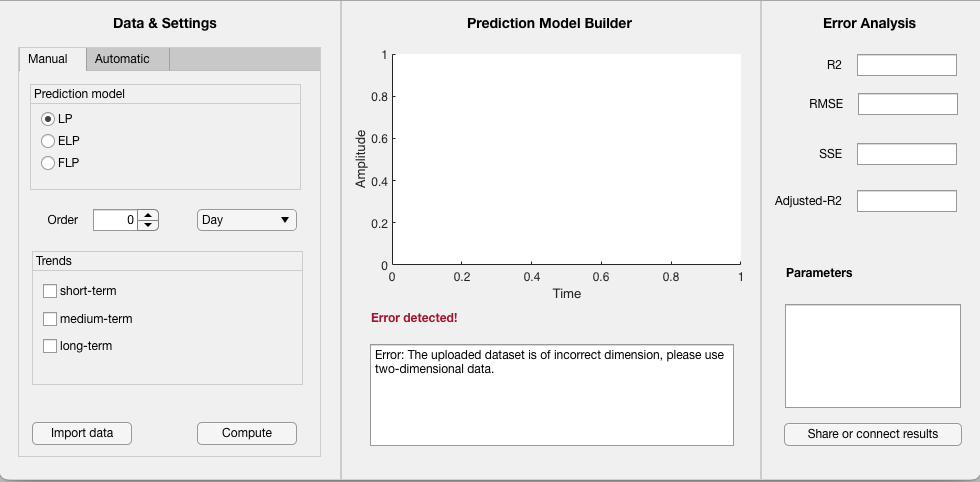
\includegraphics[width=\textwidth]{figures/warning.png}
            \caption{Dataset warning}
            \label{fig:warning}
    \end{figure}

        
        \subsection{Settings}\label{subsec:setting}
        The developed application has two main possibilities of settings, one can decide to choose a mathematical model and set other related parameters manually (Fig.~\ref{fig:manual}), or to choose automatic settings (Fig.~\ref{fig:automatic}) of application to detect the best prediction model
        based on uploaded dataset.\\
        \\
        \textbf{Manual settings}\\
     In the \emph{Manual settings} environment one is allowed to choose a prediction model (one among three) based on the type of linear prediction and to set two other settings:
  %
       \begin{figure}[h!]
        \centering
	   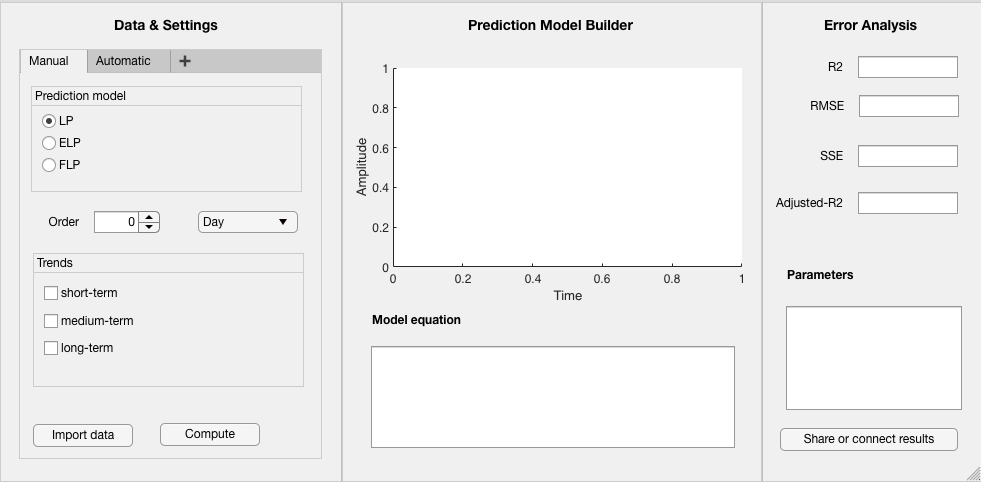
\includegraphics[width=\textwidth]{figures/manual.png}
            \caption{Manual settings}
            \label{fig:manual}
    \end{figure}



        \begin{itemize}
            \item \textbf{Prediction models}\\
            One can choose one of three types of linear prediction, \emph{Standard linear prediction}~\ref{eg:lp}, \emph{Extended linear prediction}~\ref{eg:elp},
            and \emph{Fractional-order linear prediction}~\ref{eg:flp}.\\
      \\
     The Standard linear prediction can be defined as:
     % 
                 \begin{equation}\label{eg:lp}
                \hat{x}(n) = \sum_{i=1}^{p} a_i x(n-i),
                \label{eq:linear-predictor}
            \end{equation}
              %
            where $\hat{x}(n)$ is the~predicted value of $x(n)$, $p$ is the~order of the~predictor, and $a_i$ are the~predictor coefficients. The~predictor coefficients can be found by minimizing the~prediction error.
                        \\
                        \\
    The Extended linear prediction can be defined as:
%
                 \begin{equation}\label{eg:elp}
                \hat{x}(n) = \left(\sum_{i=1}^{p} a_i x(n-i) + \sum_{i=1}^{q} b_i x(n-S-i)\right) * \gamma(n),
            \end{equation}
           %
            where $\hat{x}(n)$ is the~predicted value of the~order at time $n$, $x(n-i)$ is the~past short-therm prediction part $p$ samples of the~dataset, $x(n-S-i)$ is the~past long-term prediction part with seasonal shift $S$, and $a_i$ and $b_i$ are the~predictors coefficients. The~order of the~predictor is $p$ for short-term and $q$ for the long-term linear prediction. The seasonal weights are represented by $\gamma(n)$.\\
                                    \\
    The Fractional-order linear prediction can be defined as:
            \\
            \begin{equation}\label{eg:flp}
                \hat{x}(n) = \frac{a}{h^\alpha}(x(n-1) - \alpha x(n-2)),
                \label{eq:linear-predictor}
            \end{equation}
            %
            that uses two-samples memory, is dependent on one parameter $a$ and the order of fractional derivative $\alpha$~CITE T. Skovranek, V. Despotovic and Z. Peric, "Optimal Fractional Linear Prediction With Restricted Memory," in IEEE Signal Processing Letters, vol. 26, no. 5, pp. 760-764, May 2019, doi: 10.1109/LSP.2019.2908278.
.
           
            \item \textbf{Prediction order}\\
            In this step we are able to set up the order of linear prediction and the
            period of predicted values.
            \item \textbf{Trends detection}\\
            In this setting you are able to choose the length of the period to 
            identify the prediction model parameters and trends.
        \end{itemize}
        \noindent
        \\
        \textbf{Automatic settings}\\
        The \emph{Automatic settings} can be used to set up the parameters of neural network,
        which is used to estimate optimal parameters for prediction. 
                  %
       \begin{figure}[h!]
        \centering
            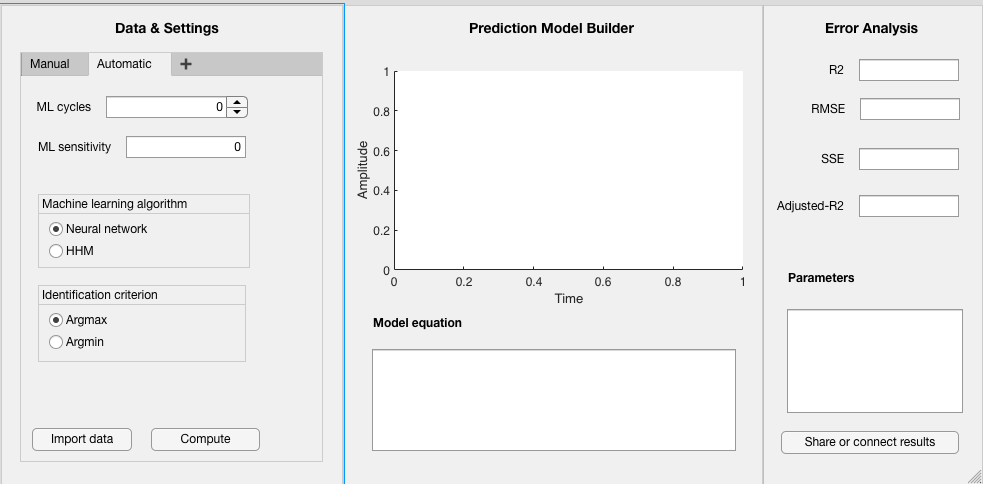
\includegraphics[width=\textwidth]{figures/auto.png}
            \caption{Automatic settings}
            \label{fig:automatic}
    \end{figure}
        %
                For the set up of automation part of application we are able to use these parameters:\\
        \begin{itemize}
            \item \textbf{Machine learning cycles}\\
            Number of observations used to find optimal parameters of the model.
            \item \textbf{Machine learning sensitivity}\\
            Sensitivity is a measure of how well a machine learning model can
            detect positive instances. It is also known as the true positive rate
            (TPR) or recall.
            \item \textbf{Machine learning algorithms}\\
            In this section we are able to choose the neural network or hidden Markov model
            to run in background. HMM is statistical approach and in specific dataset can provide
            better results.
            \item \textbf{Identification criteria}\\
            In this part we can choose the maximisation or minimisation as the criterion
            to find optimal parameters.
        \end{itemize}
   
        \subsection{Results}\label{subsec:result}
        For the test purpose, we used the automatic settings of the application and run the application with the uploaded
       dataset. Figure~\ref{fig:results} shows the results of the developed application.
       %
               \begin{figure}[h!]
        \centering
            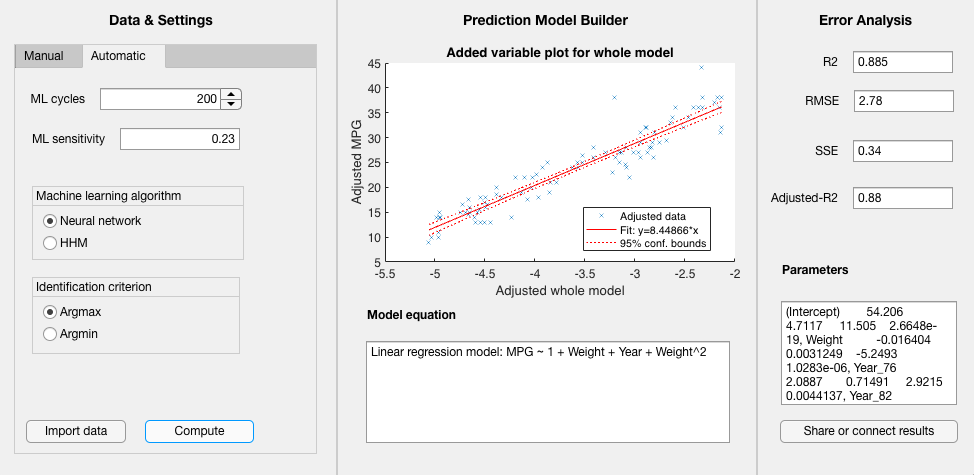
\includegraphics[width=\textwidth]{figures/result.png}
            \caption{Results}
            \label{fig:results}
    \end{figure}
        %
        Application successfully detects the model equation, identifies optimal parameters and 
        calculates the fitting criteria. Model builder creates the model with $R^2 = 0.885$.
        The application displays the results in these four sections:\\
        \\
        \textbf{Plot of results}\\
       Figure~\ref{fig:results} shows the main window of the application, where in the middle of the screen
       the uploaded dataset as well as the moddeled fitting-curve are plotted.\\
        \\
        \textbf{Model equation}\\
        Under the main section with plotted results, one can find the model equation section, where
       the mathematical model proposed by the application is shown.\\
        \\
        \textbf{Parameters}\\
        In the right bottom corner one can see the parameters of the identified model. When the
        Model equation and Parameters section are combined, we are able to use the created model in other
        applications and approaches if necessary.\\
        \\
        \textbf{Error Analysis}\\
        The last part of the application is Error Analysis, where we can find the 
        results of the created model. Application provides $R^2$, adjusted $R^2$,
        Root Mean Square Error and Sum Squared Error.
        
        